\chapter{Marco Te\'orico}

%%%%%%%%%%%%%%%
%%%%%%%%%%%%%%%
\section{first}

%%%%%%%%%%%%%%%
\subsection{first-1}
Esto es un ejemplo de referencia \cite{STRO01}. Esto es un ejemplo de c\'odigo en pseudoformal:


\begin{algorithmic}[upquote=true, language=pseudo]
	\Require $n \geq 0$
	\Ensure $y = x^n$
	\State $y \Leftarrow 1$
	\State $X \Leftarrow x$
	\State $N \Leftarrow n$
	\While{$N \neq 0$}
	\If{$N$ is even}
	\State $X \Leftarrow X \times X$
	\State $N \Leftarrow \frac{N}{2} $  \Comment{This is a comment}
	\ElsIf{$N$ is odd}
	\State $y \Leftarrow y \times X$
	\State $N \Leftarrow N - 1$
	\EndIf
	\EndWhile
\end{algorithmic}
%%%%%%%%%%%%%%%
%%%%%%%%%%%%%%%
\section{second}

Las tablas, se pueden hacer con \url{https://www.tablesgenerator.com} y referenciarlos \ref{lb:table1}.

\begin{table}[htpb!]
	\centering
	\begin{tabular}{ll}
		Value & Description         \\
		3     & None to say         \\
		2     & Fill with something
	\end{tabular}
	\caption{Irrelevant data}
	\label{lb:table1}
\end{table}

%%%%%%%%%%%%%%%
\subsection{second-1}
Las referencias tambi\'en pueden hacerse en conjunto \cite{REF_MIC,WEB99}.



\noindent Aqu\'i las otras referencias \cite{RAM11}

\subsubsection{second-1-1}

Para insertar im\'agenes, hay diversos enfoques (incluyendo subfigure) \ref{fig:reloj}.

\begin{figure}[htpb!]
	\centering
	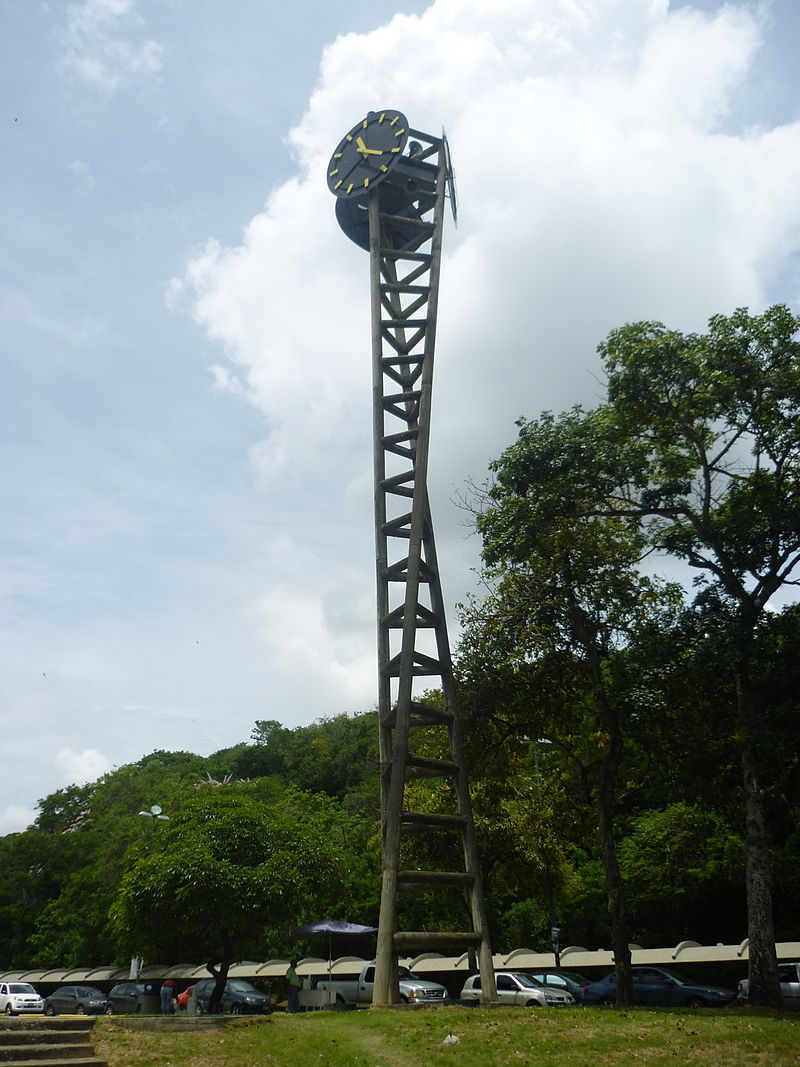
\includegraphics[width=0.5\columnwidth]{images/reloj.jpg}
	\label{fig:reloj}
	\caption{Reloj sin chichero}
\end{figure}

